%!TEX root = ../bachelorthesis.tex
\chapter{Evaluierung}
\label{chap:evaluierung}
In diesem Kapitel wird die Durchführung einer robotergestützten Kalibrierung beschrieben. Zusätzlich wird diese Durchführung mit einer manuellen Kalibrierung verglichen. Einen Überblick über den Aufbau geben \autoref{img:experiment_camera} und \autoref{img:experiment_side}.
\begin{figure}
\centering
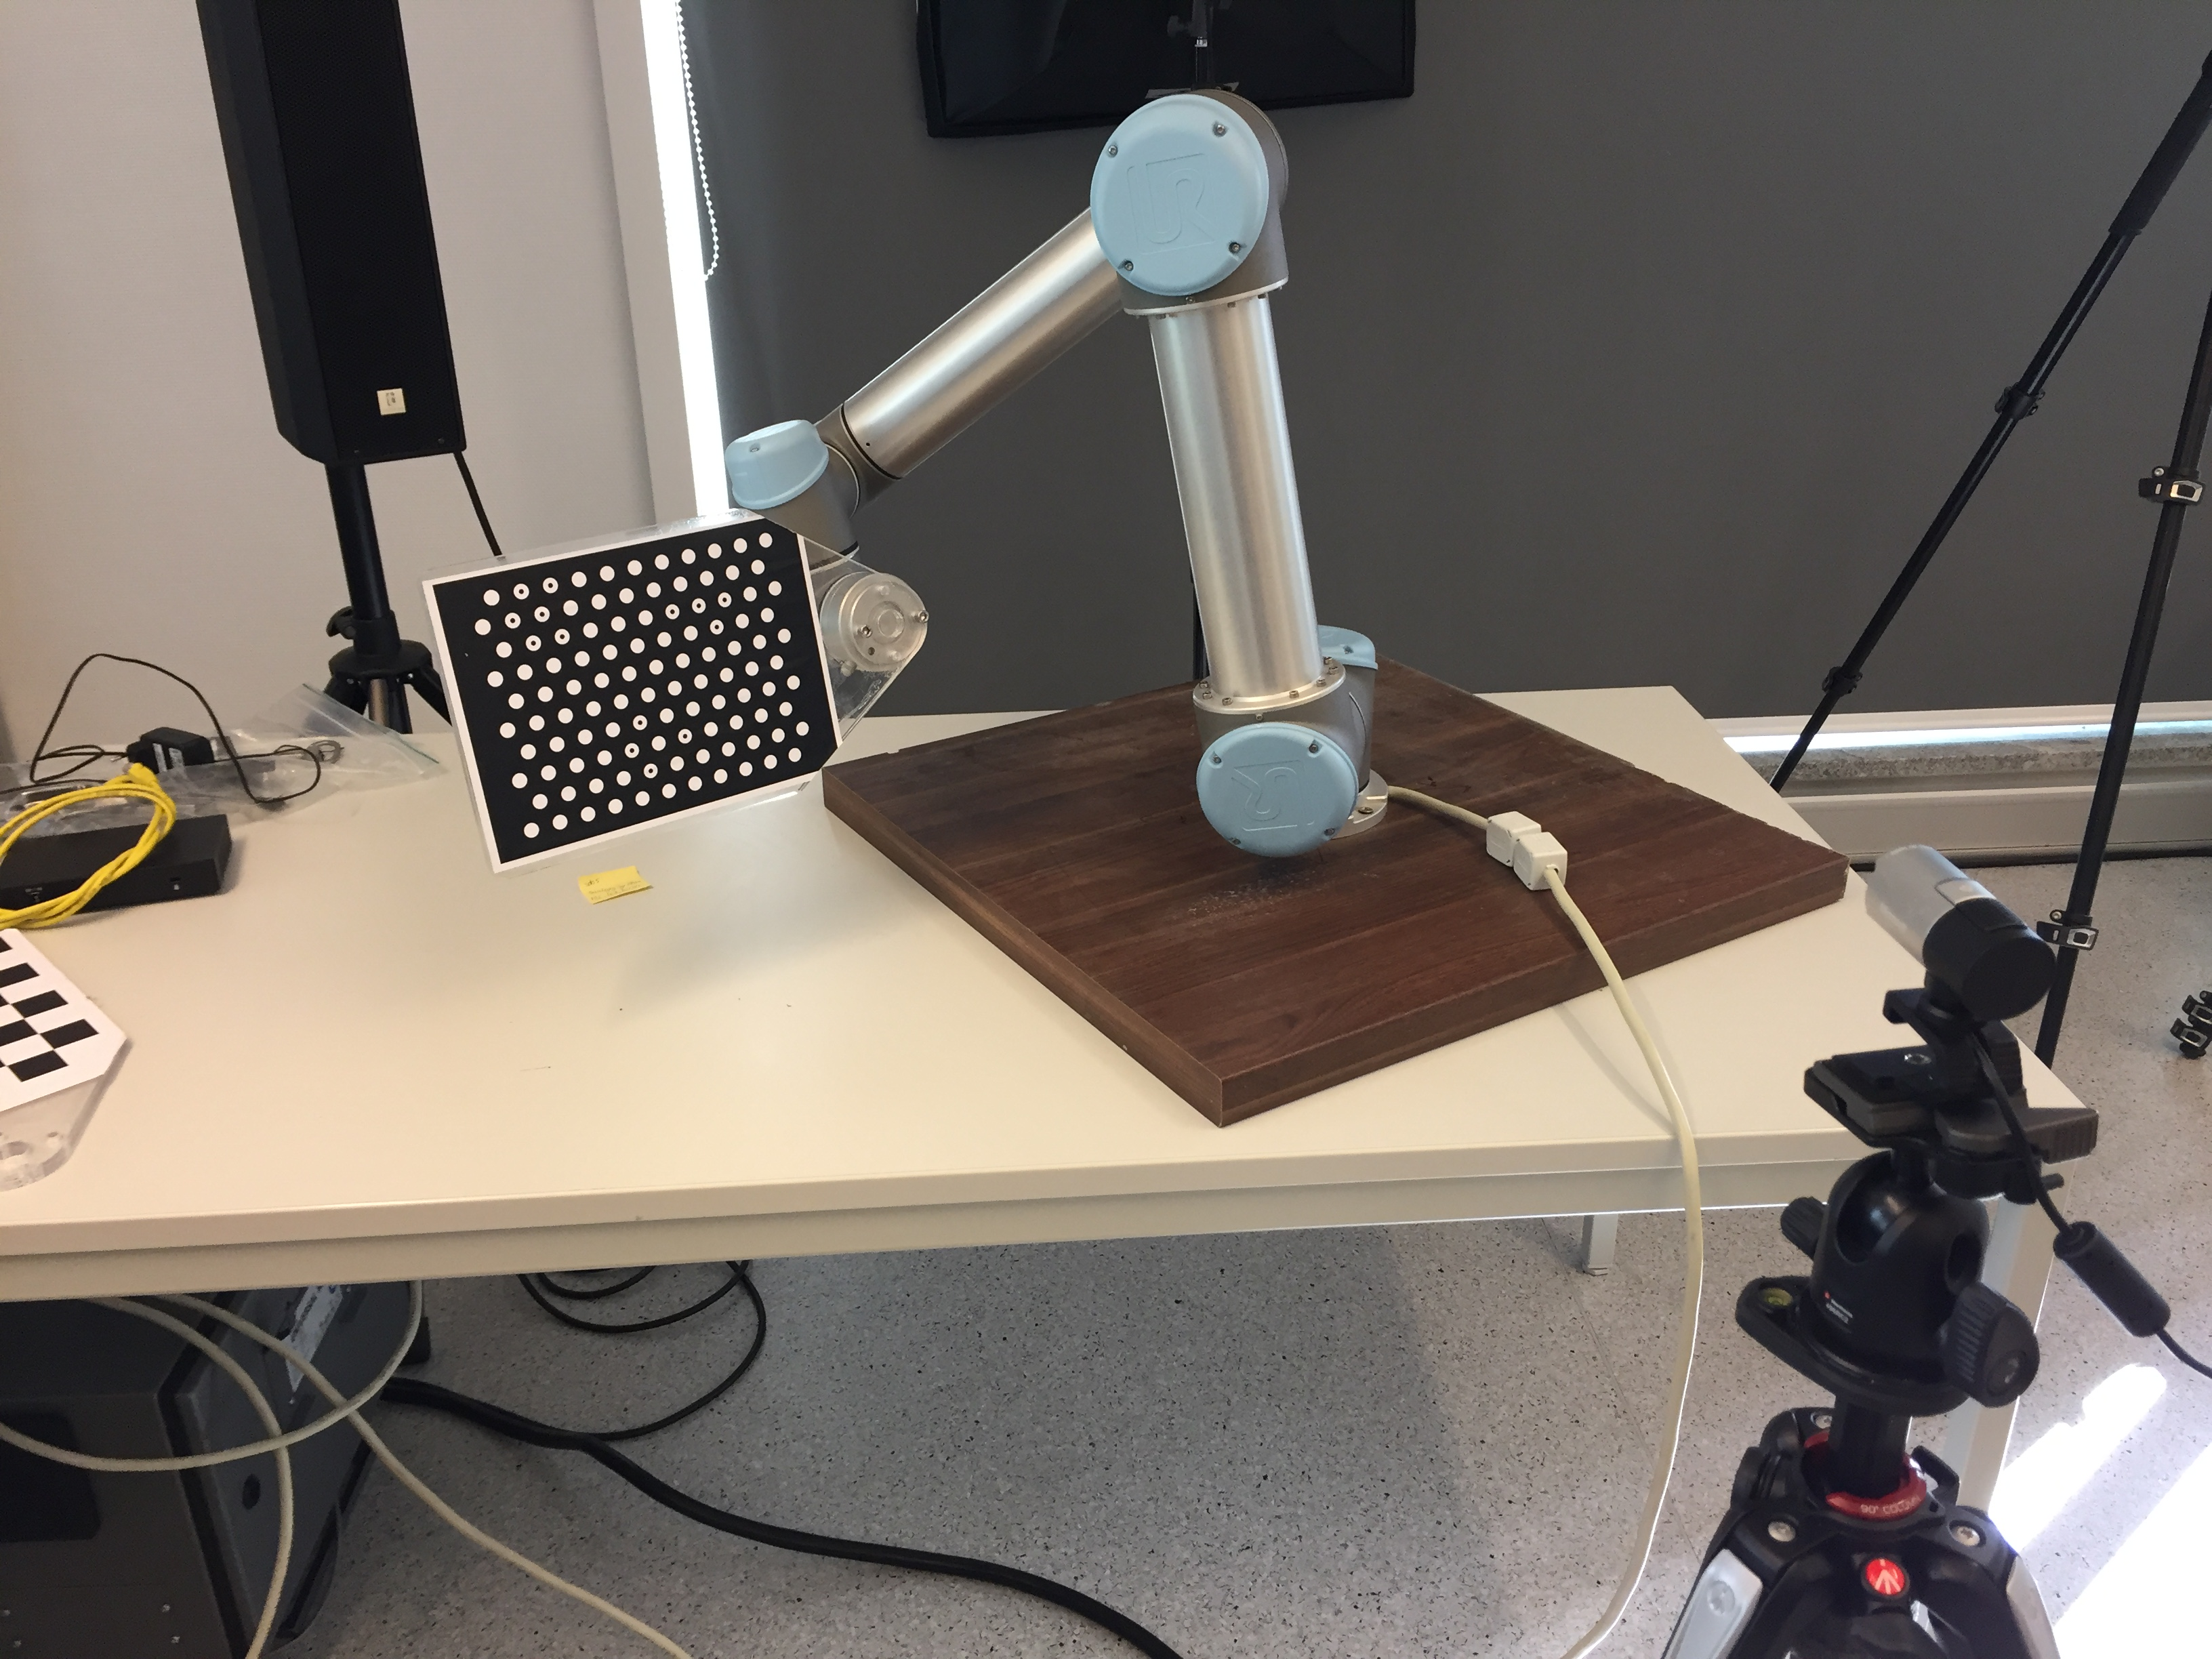
\includegraphics[width=0.8\textwidth]{images/experiment_camera.JPG}
\caption{Der Aufbau zur Kalibrierung aus Sicht der Kamera.}\label{img:experiment_camera}
\end{figure}
\begin{figure}
\centering
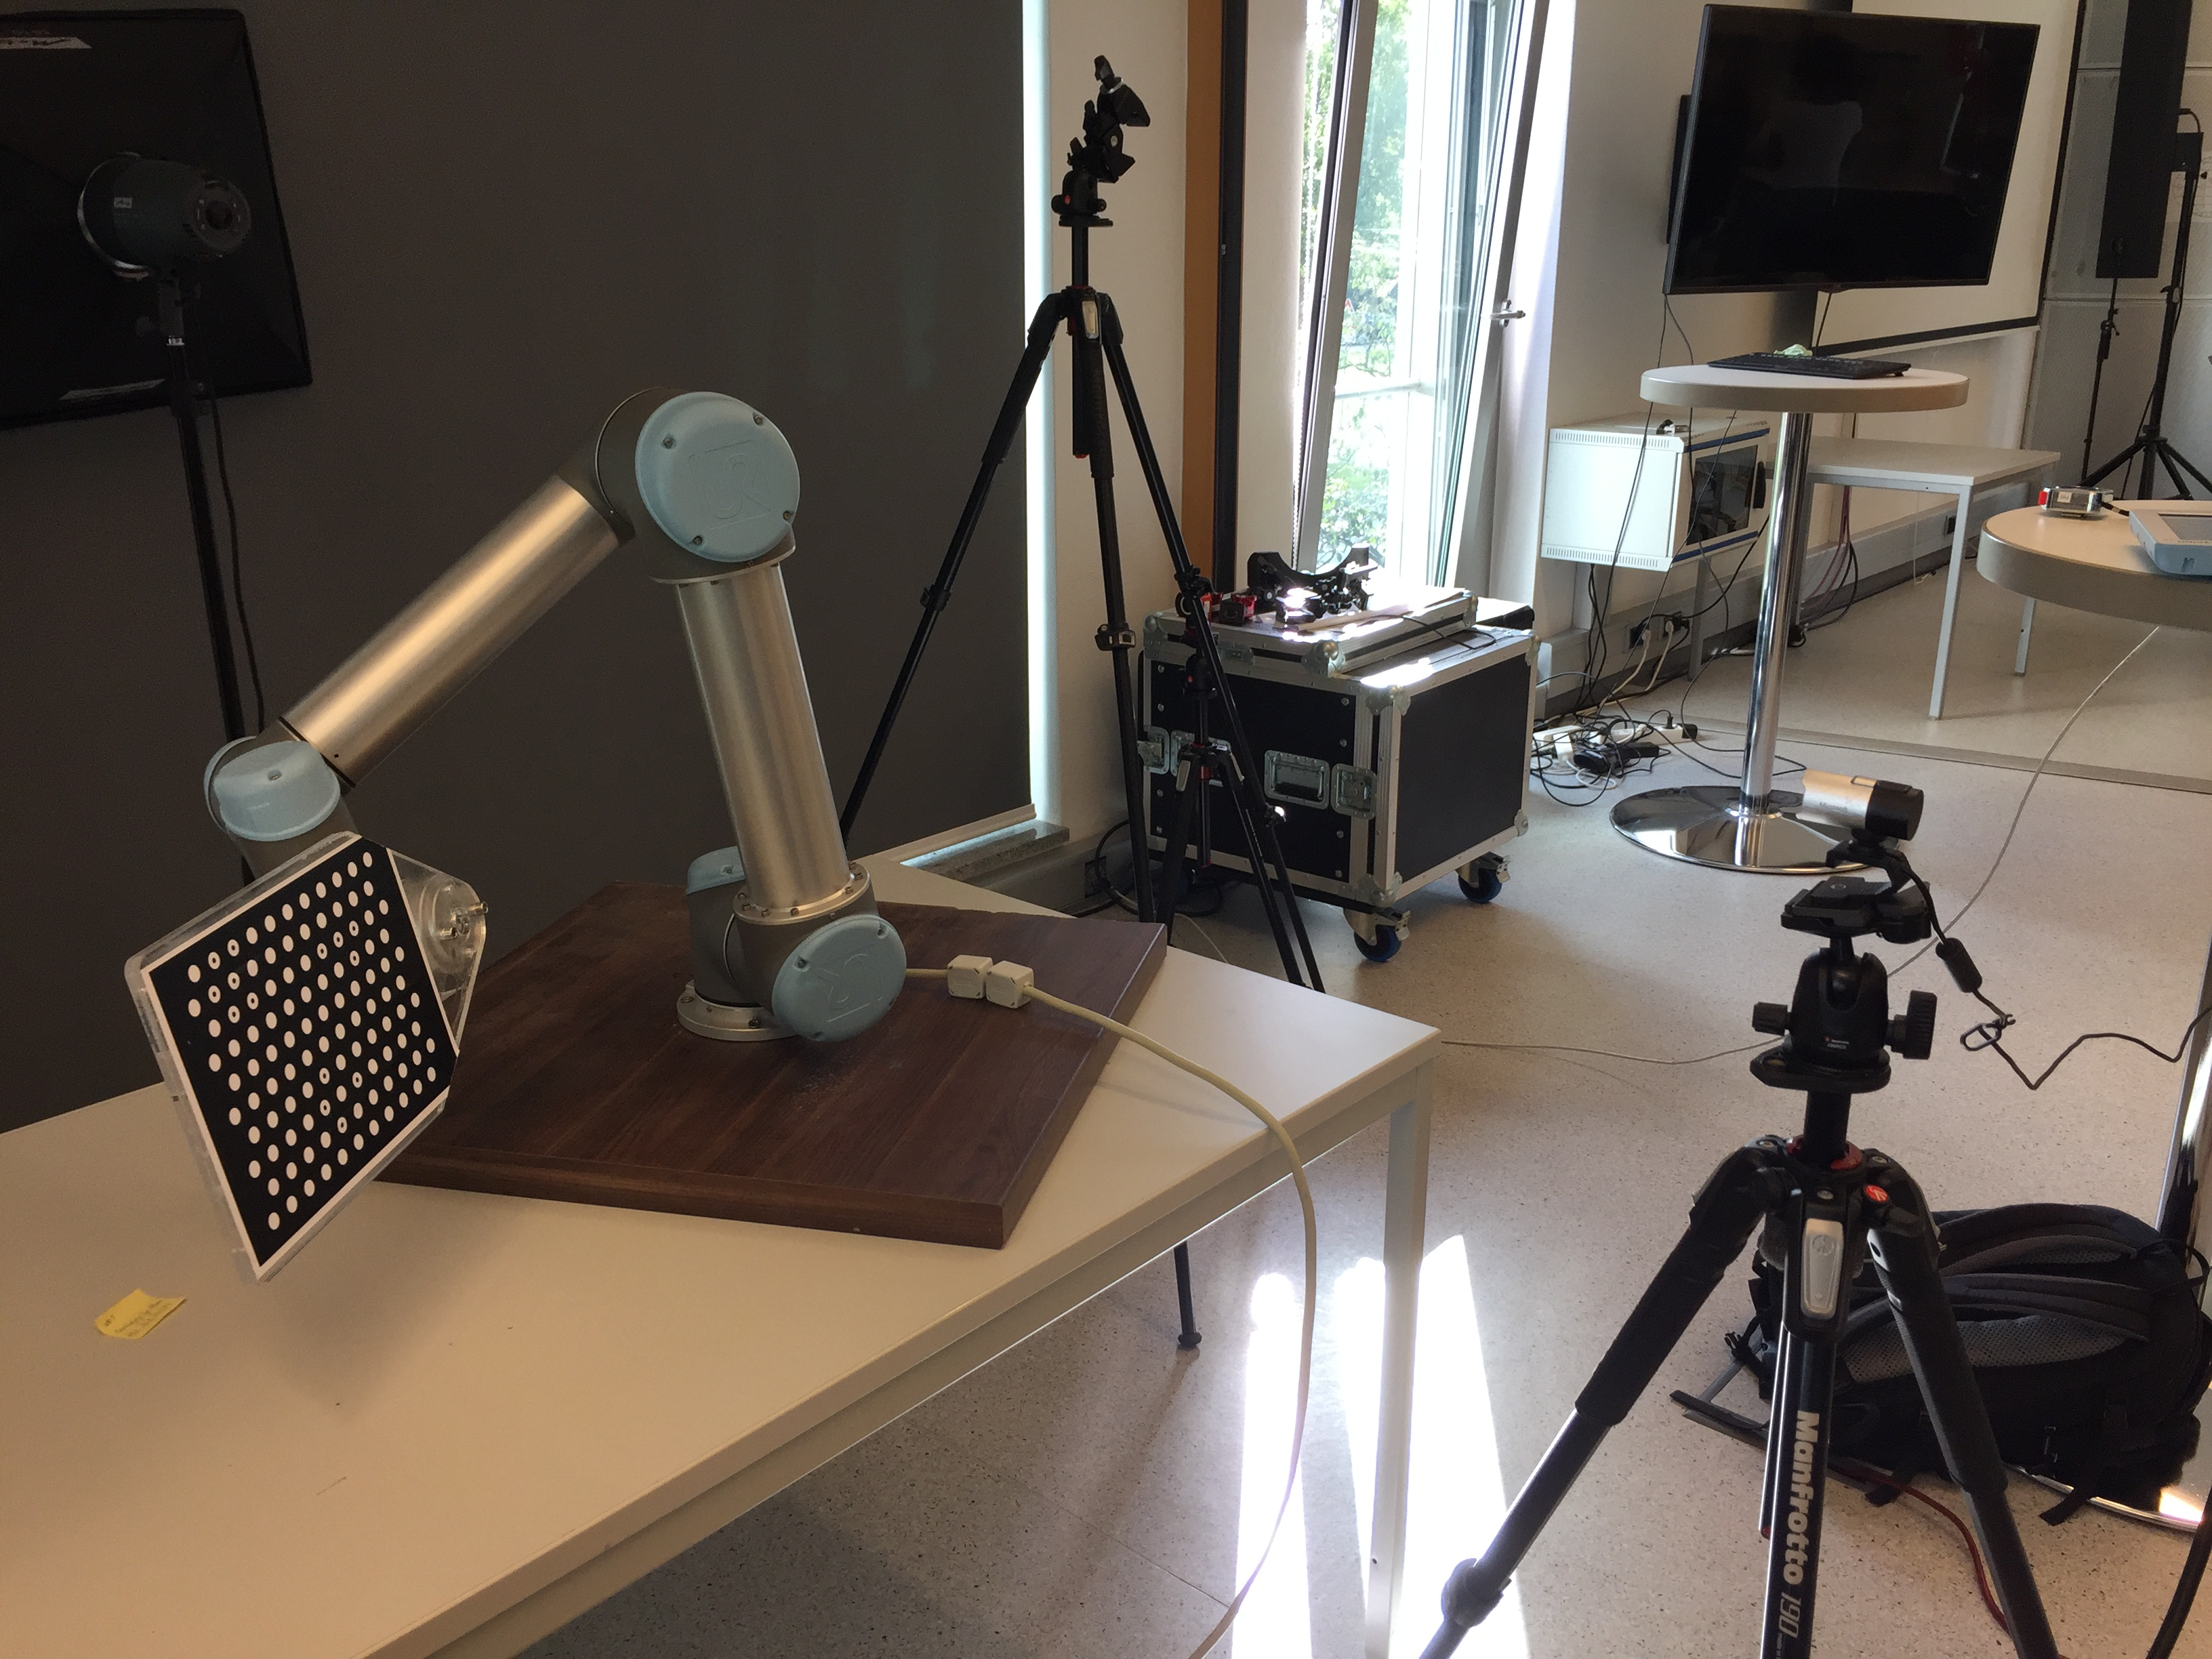
\includegraphics[width=0.8\textwidth]{images/experiment_side.JPG}
\caption{Der Aufbau zur Kalibrierung von der Seite betrachtet.}\label{img:experiment_side}
\end{figure}

Die Kalibrierung wurde mit den folgenden Komponenten durchgeführt: Als Kamera wurde die Microsoft LifeCam Studio benutzt. Sie bietet ein Farbbild mit einer Auflösung von 1920x1080 Pixeln an. Der Sensor hat laut Datenblatt eine Höhe von 3,27 mm und eine Breite von 5,85 mm. Die Brennweite beträgt 3,7 mm. Als Roboter wird der UR5 von Universal Robotics eingesetzt. Als Kalibrierungsmuster wird das Muster aus \autoref{img:caltab_hex_10x11} benutzt. Es wurde auf DinA4-Größe gedruckt.

Die Kamera steht von der Basis des Roboters aus gesehen an der Position x=-0,95, y=0 und z=0.35. Die Kamera ist so ausgerichtet, dass der Mittelpunkt des Bildes ungefähr mittig über der Basis in einer Höhe von 45 cm liegt. Die weiteren Parameter wie die Faktoren zur Distanzbestimmung oder die Verzögerung zwischen dem Erreichen einer Position und der Aufnahme des Bildes werden nicht verändert.

Der UR5-Roboter muss über das angeschlossene Tablet gestartet werden. Zusätzlich muss die IP-Adresse für den Roboter bekannt sein. Auch die Kamera muss über USB mit dem Rechner verbunden sein.

Zunächst werden die Nodes zur Steuerung des Roboters gestartet, beginnend mit dem Hardware Driver. Die IP-Adresse ist selbstverständlich spezifisch für dieses Szenario.
\begin{lstlisting}[language=bash]
  $ roslaunch ur_modern_driver ur5_bringup_joint_limited.launch robot_ip:=192.168.102.95
\end{lstlisting}
Die zweite Node startet MoveIt!.
\begin{lstlisting}[language=bash]
  $ roslaunch roslaunch ur5_moveit_config ur5_moveit_planning_execution.launch limited:=true
\end{lstlisting}
Die dritte Node startet RViz, um die Planning Scene visuell überprüfen zu können:
\begin{lstlisting}[language=bash]
  $ roslaunch ur5_moveit_config moveit_rviz.launch config:=true
\end{lstlisting}

Damit sind die Nodes gestartet, um den Roboter bewegen zu können. Damit MoveIt! über Hindernisse in der Umgebung, wie zum Beispiel der Tisch oder Wände, informiert ist, wird die Node \texttt{publish\_collision\_objects} gestartet. In dieser sind die geometrischen Informationen über die Umgebung gespeichert. Ändert sich die Umgebung, muss auch diese Node angepasst werden.
\begin{lstlisting}[language=bash]
  $ rosrun robot_assisted_calibration publish_collision_objects.py
\end{lstlisting}

Um die Bilder der Kamera in ROS zu veröffentlichen, wird ein weiteres launchfile gestartet. Diese gehört nicht zu einen ROS-Paket, daher muss es aus dem Verzeichnis gestartet werden, in dem es liegt, in diesem Fall im Order libuvc: \todo{In das robot-assisted-calibration Paket verschieben}
\begin{lstlisting}[language=bash]
  $ cd libuvc
  $ roslaunch camera.launch
\end{lstlisting}

Nun sind alle Hardware-spezifischen Nodes gestartet, sodass nun die Programme zur Kalibrierung gestartet werden können. Es wir mit der Node begonnen, die das maschinelle Sehen übernimmt. Hier ist zu beachten, dass in diesem Fall im aktuellen Verzeichnis ein neuer Ordner erstellt wird, in dem die Bilder gespeichert werden. Soll dieser Ordner in einem anderen Verzeichnis erstellt werden, muss dieses Verzeichnis über den Parameter \texttt{image\_path:=/Pfad/Zum/Verzeichnis} angegeben werden.
\begin{lstlisting}[language=bash]
  $ roslaunch caltab_detector caltab_detector.launch
\end{lstlisting}

Als nächstes wird die Node gestartet, die die Befehle an MoveIt! übermittelt. Dies passiert mit dem folgenden Befehl:
\begin{lstlisting}[language=bash]
  $ rosrun robot_assisted_calibration MoveArmServer.py
\end{lstlisting}

Schließlich wird der CalibrationController gestartet, der direkt mit der Kalibrierung beginnt:
\begin{lstlisting}[language=bash]
  $ roslaunch robot_assisted_calibration calibration_controller.launch
\end{lstlisting}

Das Bewegen des Roboterarms an die errechneten Positionen und das Auswerten der Bilder dauert ungefähr 15 Minuten. Dabei wurden \todo{???} Positionen erreicht. Insgesamt wurden \todo{???} Bilder aufgenommen. Die Ergebnisse für diese Kalibrierung sind: \todo{???}

Da alle bis auf eine Position erreicht wurden, kann man sich ziemlich sicher sein, dass das ganze Sichtfeld und auch verschiedene Distanzen abgedeckt wurden. 

Will man eine ähnlich gute Abdeckung von Hand erreichen, wird die Aufnahme der Fotos ungefähr eine Stunde dauern. Außerdem muss man bei der manuellen Aufnahme der Fotos selber darauf achten, dass das ganze Bild exploriert wurde und ausreichend viele unterschiedliche Orientierungen und Distanzen gewählt wurden. Durch den Einsatz des Roboters hat man also nicht nur einen Zeitvorteil, sondern man kann auch die Qualität der Aufnahmen besser abschätzen.